\chapter{Deep Versat Software Simulator}
\label{chapter:Simulator}

The need for a software simulator comes from the complexity of the configurations being written into Versat and
the hardware simulation faults of being slow.

The goal is to emulate what the hardware is doing much more efficienctly than 
a simple Hardware simulation as the time of development for hardware
is much higher than simple software. The Simulator executes clock iteration per iteration 
getting the same results in each clock as the hardware. As Versat is a CGRA, different functional
unit configurations are easy to accomplish in the simulator and the time to get results on performance
for a specific program is a lot quicker. The only thing the Simualator can't do is predict
if the hardware configurations fits the FPGA that is going to be used and the clocks that 
the hardware can run. But, the propagation time is predictable depending on the number of functional units
as the difference between times in different setups is due to the multiplexers on the inputs of the FUs.

\section{Architecture and Object Relation}

The Simualtor is made up by the Parent Class called Versat, in which will be simulated itself, 
as each Versat instance is independent from each other, the simulations are also independent.
The Versat is made up of 2 CStage Arrays, one is the "live" while the other is the 
shadow registers, where the configurations are held before the simulator is ran.
Each Stage is made up of it's Functional Units, in which each one is connected to the Databus.
As it happens in the hardware, functional units can access the databus which has the output 
of the current stage and previous one.
\clearpage

\begin{figure}[!htbp]
    \centering
    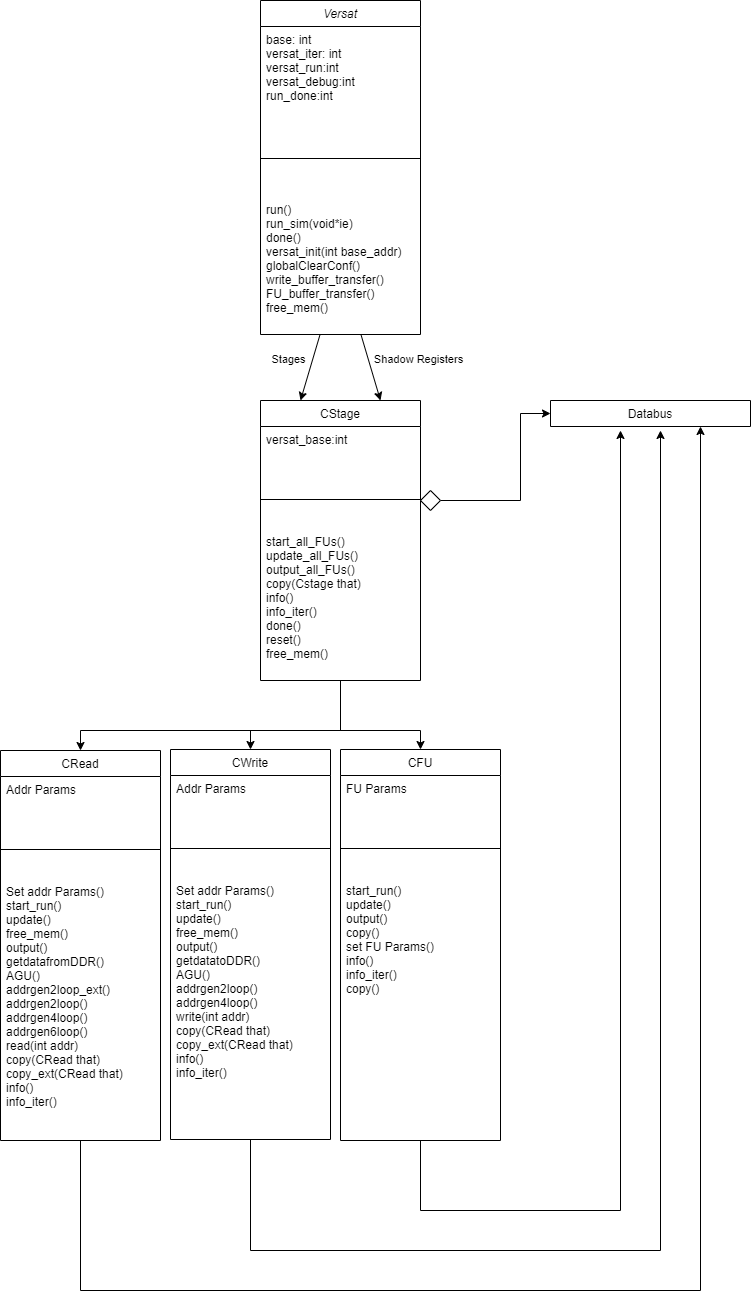
\includegraphics[width=0.8\textwidth]{Figures/VersatSimulatorDraw.drawio.png}
    \caption{Class Structure for the Versat Simulator}
    \label{figure:VersatSimulatorClass}
\end{figure} 


\section{Software API}


\section{Simulation}


